\section{Java EE und Microservices}
Aus rein technologischer Sicht bietet Java EE alles, was für eine Microservice-basierte Architektur erforderlich ist. Das wird klar, wenn die verfügbaren APIs betrachtet werden \cite{jaxcenter.2016}. Microservices ergeben sich unter Berücksichtigung folgenden Eigenschaften, welche zudem Indikatoren für die Größe darstellen \cite{EberhardWolff.2015}.
\begin{itemize}
	\item Teamgröße
	\item Modularisierung
	\item Ersetzbarkeit
	\item Transaktionen und Konsistenz
	\item Infrastruktur
	\item Verteilte Kommunikation	
\end{itemize}

\\ \\Soll ein Microservice mit Java EE implementiert werden, lassen sich diese Indikatoren ebenfalls heranziehen. Die Anzahl der Teammitglieder beschränkt die Größe der Komponente. Sie beinhaltet dabei so viel Logik, dass sie von einem Team entwickelt und betrieben werden kann. Microservices sollen eine geschlossene Fachlichkeit abbilden (Bounded Context), um sich eindeutig von anderen Services abzugrenzen. Durch diesen fachlich orientierten Aufbau, lässt sich der Dienst unabhängig von anderen Teams implementieren, testen und in Produktion bringen. Auch die Komplexität ist handhabbar, wenn der Service als Modul entwickelt wird. Dadurch lässt er sich auch ersetzen, sollte dies von Nöten sein. Die Transaktion, welche die ACID-Eigenschaften verfolgt, kann ebenfalls implementiert werden. Die Kommunikation über leichtgewichtige Mechanismen ergibt sich durch diesen Ansatz \cite{EberhardWolff.2015}. Da sie Teil eines verteilten Systems sind, bedienen sie sich über die verteilte Kommunikation einer anderen Fachlichkeit oder stellen anderen Services die eigene zur Verfügung. \\ \\
Diesen Anforderungen genügt Java EE bereits. Microservices lassen sich mit den vorhandenen APIs problemlos erstellen. Über JAX-RS (Java API for RESTful Web Services) lässt sich die Kommunikation der Dienste realisieren. Über Bean Validation (Java EE-Standard für eine schichtenübergreifende Validierung) können Requests auf ihre Korrektheit überprüft werden. Die Nutzlast kann beispielsweise über JSON-P entsprechend umgewandelt werden, um die Übermittlung zu ermöglichen. Die fachliche Logik innerhalb des Dienstes sowie die Datenhaltung lässt sich über CDI (Context and Dependency Injection) sowie JPA (Java Persistence API) realisieren \cite{LarsRowekamp.2017d}. Selbst NoSQL-Datenbanken können über entsprechende Bibliotheken an das System angebunden werden. Auch eigene Benutzeroberflächen lassen sich in solche Anwendungen integrieren, wie es bei Microservices priorisiert wird. Durch verwenden entsprechender Features lassen sich effiziente und leichtgewichtige Architekturen realisieren \cite{jaxcenter.2016}.\\ \\
Microservice-basierte Anwendungen sind Applikationen, die sich aus einer Reihe von kleinen Komponenten zusammensetzen. Diese durchlaufen dabei alle ihre eigenen Prozesse. Somit ist ein weiterer, zu berücksichtigender Punkt, die Infrastruktur. Jede Einheit muss unabhängig deployt werden können. Hierfür gibt es die Continuous-Delivery-Pipeline, die durch eine weitgehende Automatisierung dafür sorgt, dass Software bereitgestellt werden kann. Jeder Dienst benötigt somit eine eigene Infrastruktur, um ihn ausführen zu können. Diese kann auch Datenbanken oder Application Server beinhalten \cite{EberhardWolff.2015}. Hier ergibt sich allerdings ein Problem mit Enterprise Java.

\section{Das Problem mit Java EE}
Die oben aufgeführten Punkte sind Ansätze für Continuous Delivery. Diese Disziplin erfolgt durch eine weitgehende Automatisierung entsprechender Prozesse. Das eigentliche Problem liegt nicht in der zu verwendenden Technologie bzw. dem Entwickeln. Problembehaftet ist die potenzielle Automatisierung dieser Entwicklung. Auch zur Laufzeit zeigen sich negative Auswirkungen. Das Vorgehen für Build und Deployment, welches in Java EE-Anwendungen vorgesehen ist, geht über das Zusammenpacken der Komponenten, die in einem Application Server deployt werden (siehe Abbildung \ref{fig:mp1}). Die notwendige Infrastruktur wird von diesem Server bereitgestellt \cite{LarsRowekamp.2017d}. Eine Skalierung, um anfallende Lasten auszugleichen, lassen sich schwer realisieren. Bei Anwendungen, die auf Microservices basieren, geht es um tausende Serverinstanzen mit zigtausend Deployments pro Jahr (laut Amazon sogar etliche Millionen). Die Anwendungsserver leisten nicht die benötigte Performance bzw. sind zu schwerfällig für den Overhead, welchen Java EE durch die unterstützten APIs mit sich bringt \cite{jaxcenter.2016}. Der anfallende Overhead geht aus der Arbeit von Uede et all \cite{uht.2016} hervor. Der Benchmark zeigt, dass sich hier eine Drosselung der Performance ergibt. \\ \\
Leichtgewichtige Server, die nur Bestandteile mit sich bringen, welche für den Service benötigt werden, würden Abhilfe schaffen \cite{jaxcenter.2016}. Denkbar wäre hier als erster Ansatz das separate Packen der Anwendungen, welche anschließend auf dem Server deployt werden. Durch den Server können sich die Dienste die zur Verfügung gestellte Infrastruktur teilen. Microservices sollen allerdings in einem eigenen Prozess unabhängig voneinander laufen. Diese Unabhängigkeit kann durch den eben genannten Ansatz nicht realisiert werden. Das Deployment eines Service würde das Laufzeitverhalten der anderen Dienste beeinflussen. Fällt der Server aus oder weist ein Fehlverhalten durch einen defekten Dienst auf, können die anderen Module ebenfalls nicht mehr erreicht werden \cite{LarsRowekamp.2017d}.
\begin{figure}[h!]
	\centering
	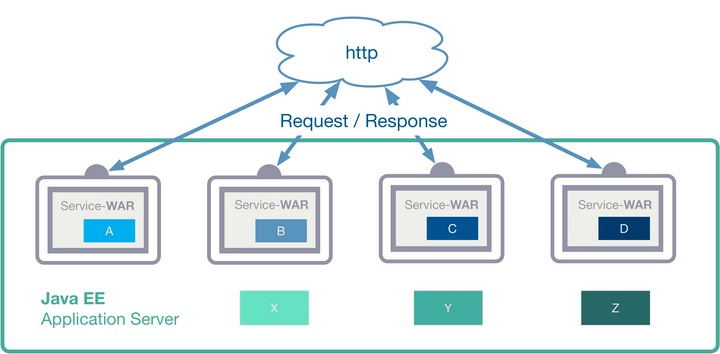
\includegraphics[width=1.0\linewidth]{images/mp1}
	\caption{Deployment in Application Server \cite{LarsRowekamp.2017d}}
	\label{fig:mp1}
\end{figure}

\section{Die Optimierung von Java EE}
Um Dienste auf Basis von Java EE bezüglich der Unabhängigkeit zu optimieren, wäre es denkbar jede Komponente in einen eigenen Server zu deployen. Jeder Dienst hat somit seine eigene Infrastruktur. Dies wird in Abbildung \ref{fig:mp2} skizziert. Wie bereits erwähnt, handelt es sich bei Microservice-basierten Systemen um etliche Service-Instanzen und deployments. Durch die angestrebte Automatisierung über die Delivery-Pipeline wären operative Aufwände wie Deployment, Konfiguration zu stemmen. Automatisierung kann beispielsweise durch das Einbetten in Docker-Images erreicht werden. Allerdings ergeben sich auch hier Probleme zur Laufzeit. Der Ressourcenverbrauch der Dienste treibt die Last auf den Servern in die Höhe \cite{LarsRowekamp.2017d}. 
\begin{figure}[h!]
	\centering
	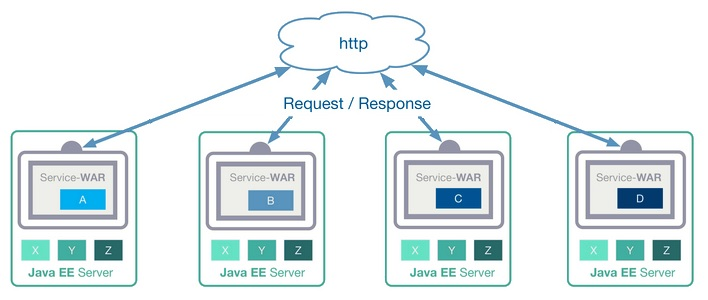
\includegraphics[width=1.0\linewidth]{images/mp2}
	\caption{Dienste mit eigener Infrastruktur \cite{LarsRowekamp.2017d}}
	\label{fig:mp2}
\end{figure}
\\ \\Führende Hersteller von Application Server sind bereits daran Lösungen zu entwickeln. Produkte in diesem Umfeld sind beispielsweise WildFly Swarm, TomEE Shades, Payara Micro. Dabei sollen die benötigten Bestandteile und Funktionalitäten des Servers in den Service eingebunden werden \cite{jaxcenter.2016}. Eine Kombination aus Server-Komponenten und Service-Geschäftslogik lassen sich daraufhin als ausführbares Programm packen. Dies wird in Abbildung \ref{fig:mp22} veranschaulicht. Ein fachlich gekapselter Service bringt so seine eigene Laufzeitumgebung mit. Diese Umgebung lässt sich auf den Service anpassen, wodurch der Overhead reduziert werden kann. Sobald dieser Service deployt wird, kann er gestartet und ausgeführt werden. Er ist autark und läuft als eigener Prozess \cite{jaxcenter.2016}. Trotz, dass mit diesem Ansatz scheinbar alle Aspekte umgesetzt wird, bleibt jedoch das Einbinden der Server-Komponenten, was den Build-Prozess verlangsamt \cite{LarsRowekamp.2017d}.
\begin{figure}[h!]
	\centering
	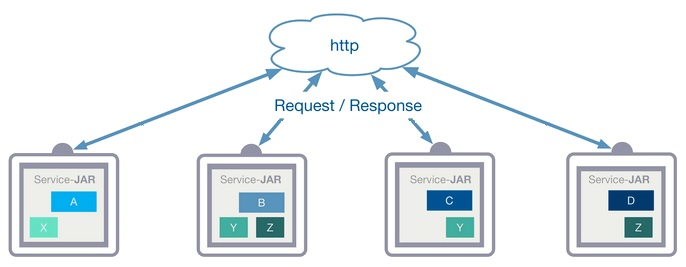
\includegraphics[width=1.0\linewidth]{images/mp3}
	\caption{Dienste mit eigener Infrastruktur 2\cite{LarsRowekamp.2017d}}
	\label{fig:mp22}
\end{figure}
\\ \\Zudem ist dieser Ansatz noch zu grobgranular. Er stellt daher weniger einen Microservice dar, es handelt sich eher um ein Self-contained System (SCS) \cite{jaxcenter.2016}. Dieser Ansatz teilt sich eine Vielzahl von Konzepten mit Microservices (Isolation, unabhängige Einheiten, fachliche Trennung, Technologiefreiheit, keine zentrale Infrastruktur), besitzt jedoch noch einige Unterschiede. Wie eben hervorgegangen ist, weist die Größe ein Unterschied auf. Ein System besitzt normalerweise weniger SCS als Microservices. Ein wichtiger Aspekt ist die Kommunikation zwischen den Komponenten. Microservices können untereinander kommunizieren. SCSs sollten dies idealerweise nicht. Auch bringen Microservices oft ihre eigene Benutzeroberfläche mit sich, während sich SCSs eine gemeinsame teilen. Es wird an dieser Stelle also nicht das gewünschte Problem gelöst. SCSs sind eher für Architekturen größerer Projekte geeignet. Sollen noch unabhängigere, kleinere Komponenten entwickelt werden, die auch mit Continuous Delivery arbeiten, muss noch ein Schritt weitergegangen werden \cite{selfcontainedservices.2017}.

 